\documentclass{beamer}

\usepackage[utf8]{inputenc}
\usecolortheme{beaver}
\usepackage{caption}
\usepackage{subcaption}
\usepackage{mathtools}
\usepackage{todonotes}
\usepackage{amsmath}
\usepackage{bm}
\usepackage{listings}
\usepackage{ragged2e}
\usepackage{titlecaps}
\usepackage{fancyvrb}

\def\ci{\perp\!\!\!\!\!\perp}

\newtheorem{proposition}{Proposition}
\Addlcwords{for a is but and with of in as the etc on to if}

\setbeamertemplate{section in toc}{\inserttocsectionnumber.~\inserttocsection}
\usetheme{Boadilla}
\makeatletter
\setbeamertemplate{footline}{%
    \leavevmode%
    \hbox{%
        \begin{beamercolorbox}[wd=.3\paperwidth,ht=2.25ex,dp=1ex,center]{author in head/foot}%
            \usebeamerfont{author in head/foot}\insertshortauthor\expandafter\beamer@ifempty\expandafter{\beamer@shortinstitute}{}{~~(\insertshortinstitute)}
        \end{beamercolorbox}%
        \begin{beamercolorbox}[wd=.55\paperwidth,ht=2.25ex,dp=1ex,center]{title in head/foot}%
            \usebeamerfont{title in head/foot}\insertshorttitle
        \end{beamercolorbox}%
        \begin{beamercolorbox}[wd=.15\paperwidth,ht=2.25ex,dp=1ex,right]{date in head/foot}%
            \usebeamerfont{date in head/foot}\insertshortdate{}\hspace*{2em}
            \insertframenumber{} / \inserttotalframenumber\hspace*{2ex} 
        \end{beamercolorbox}}%
        \vskip0pt%
    }
\makeatother

\begin{document}

\title[]{A cautious approach to constraint-based causal model selection}
\date{}

\begin{frame}
	\begin{figure}
		
\includegraphics[scale=0.3]{imgs/title.png}
	\end{figure}
\end{frame}

\begin{frame}{DAGs and Implied Conditional Independences}
	Each missing edge implies a Conditional Independence (CI) statement.

	\begin{figure}
		\centering
		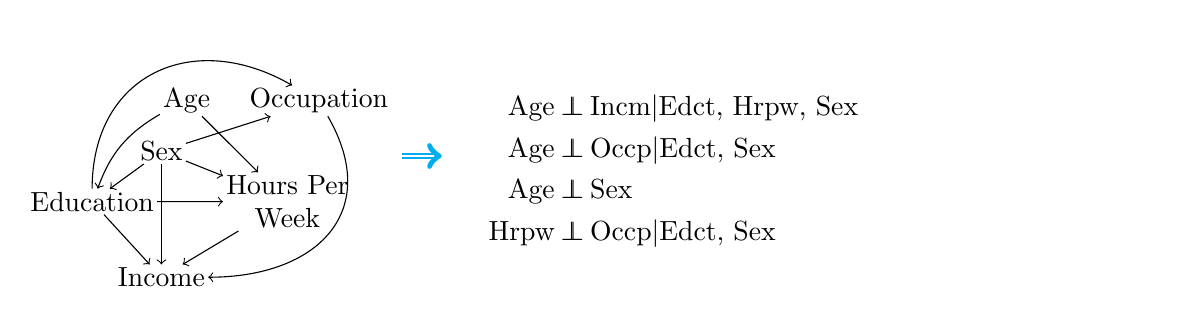
\begin{tikzpicture}
			\begin{scope}[yshift=0.7cm, scale=0.8]
			\tikzstyle{every node}=[align=center, inner sep=1pt]
				\node (sex) at (-0.7, -0.8) {Sex};
				\node (age) at (-0.3, 0) {Age};
				\node (ed) at (-1.8, -1.6) {Education};
				\node (occ) at (1.8, 0) {Occupation};
				\node (hrpw) at (1.3, -1.6) {Hours Per \\ Week};
				\node (income) at (-0.7, -2.8) {Income};
			
				\draw[->]  (age) to[bend right=20] (ed);
				\draw[->]  (sex) to (ed);
				\draw[->]  (age) to (hrpw);
				\draw[->]  (ed) to (hrpw);
				\draw[->]  (sex) to (hrpw);
				\draw[->]  (ed) to (income);
				\draw[->]  (hrpw) to (income);
				\draw[->]  (occ) to[out=300, in=0, looseness=1.4] (income.east);
				\draw[->]  (sex) to (income);
				\draw[->]  (ed) to[out=90, in=150, looseness=1.3] (occ);
				\draw[->]  (sex) to (occ);	
			\end{scope}
			\draw[thick, ->, double, cyan] (2.5,0) -- (3,0);
			\node[rectangle, align=center, inner sep=1pt] at (6, 0) {
				\begin{minipage}{\textwidth}
					\begin{equation*}
						\begin{split}
							\textnormal{Age} &\ci \textnormal{Incm} \rvert \textnormal{Edct, Hrpw, Sex} \\
							\textnormal{Age} &\ci \textnormal{Occp} \rvert \textnormal{Edct, Sex} \\
							\textnormal{Age} &\ci \textnormal{Sex} \\
							\textnormal{Hrpw} &\ci \textnormal{Occp} \rvert \textnormal{Edct, Sex} \\
						\end{split}
					\end{equation*}
				\end{minipage}
				};
		\end{tikzpicture}
	\end{figure}
	\vspace{1em}
	Datasets generated from this DAG should also satisfy these CIs (faithfulness).

\end{frame}

\begin{frame}{Constraint-Based Structure Learning}
	\center Constraint-based algorithms utilize CIs in data to learn DAGs.
	%\begin{figure}
	%	\centering
	%	\begin{tikzpicture}
	%		\begin{scope}
	%			\tikzstyle{every node}=[align=center, inner sep=1pt]
	%			\node (x1) at (0, 0) {$ X_1 $};
	%			\node (x2) at (0, -1) {$ X_2 $};
	%			\node (x3) at (1, -1) {$ X_3 $};
	%			\node (x4) at (1, 0) {$ X_4 $};

	%			\draw[->] (x1) to (x3);
	%			\draw[->] (x2) to (x3);
	%			\draw[->] (x3) to (x4);
	%		\end{scope}
	%		\begin{scope}[xshift=2cm]
	%			\draw[->] (0, -0.5) to (1, -0.5);
	%		\end{scope}
	%	\end{tikzpicture}
	%\end{figure}
	\begin{figure}
		\centering
		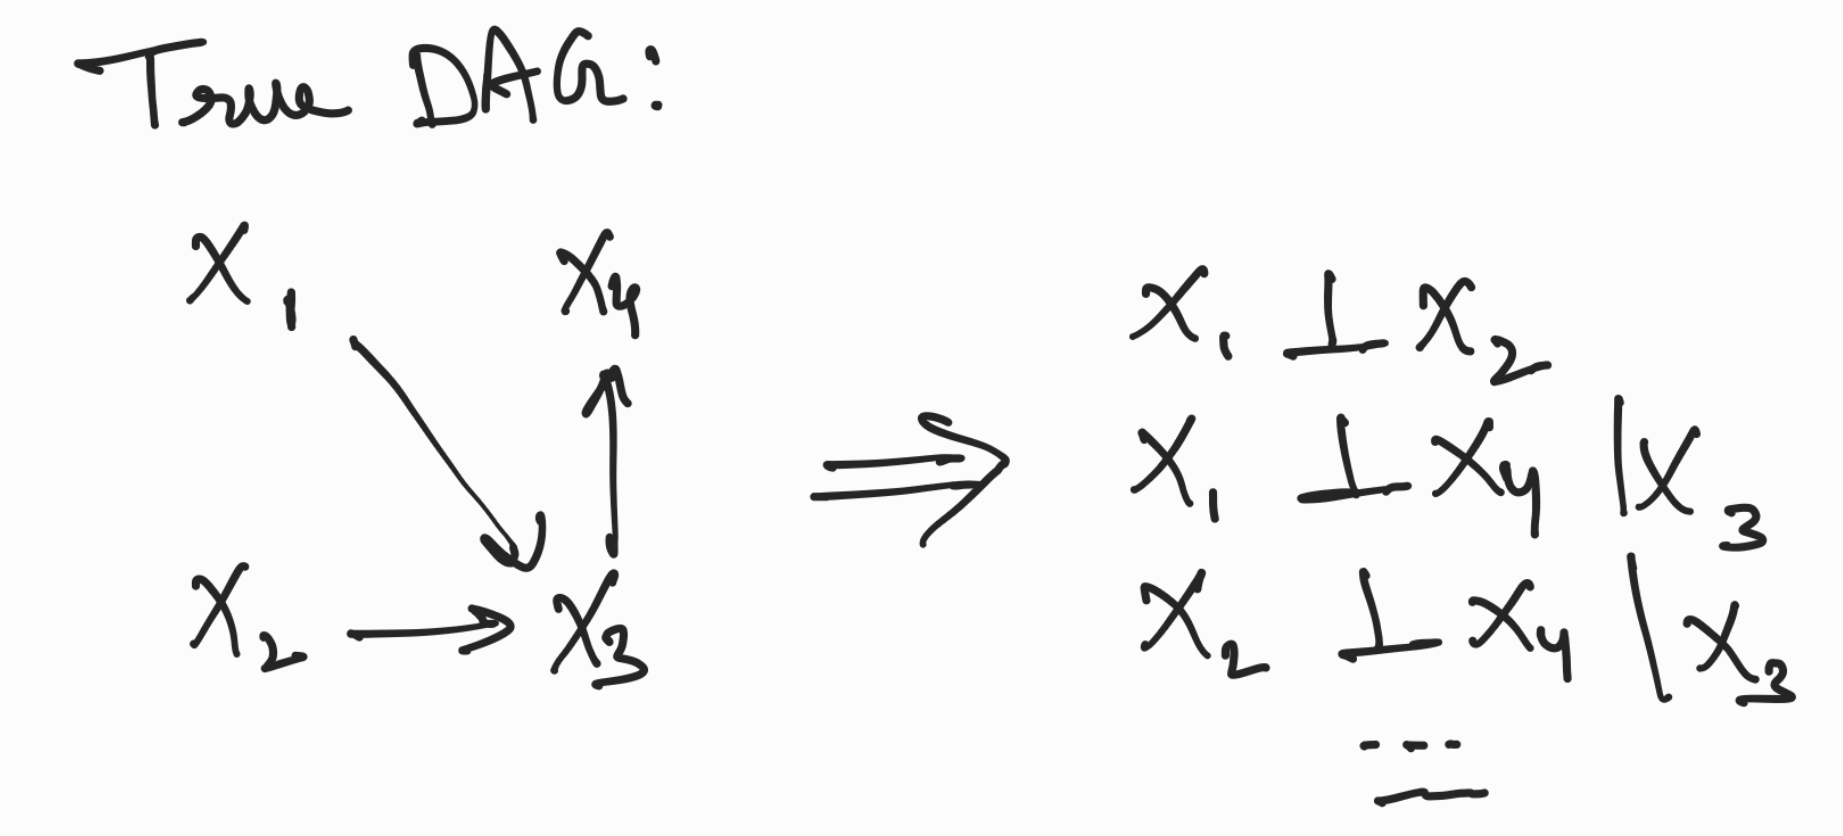
\includegraphics[scale=0.12]{imgs/example1.png}
	\end{figure}
	\begin{figure}
		\centering
		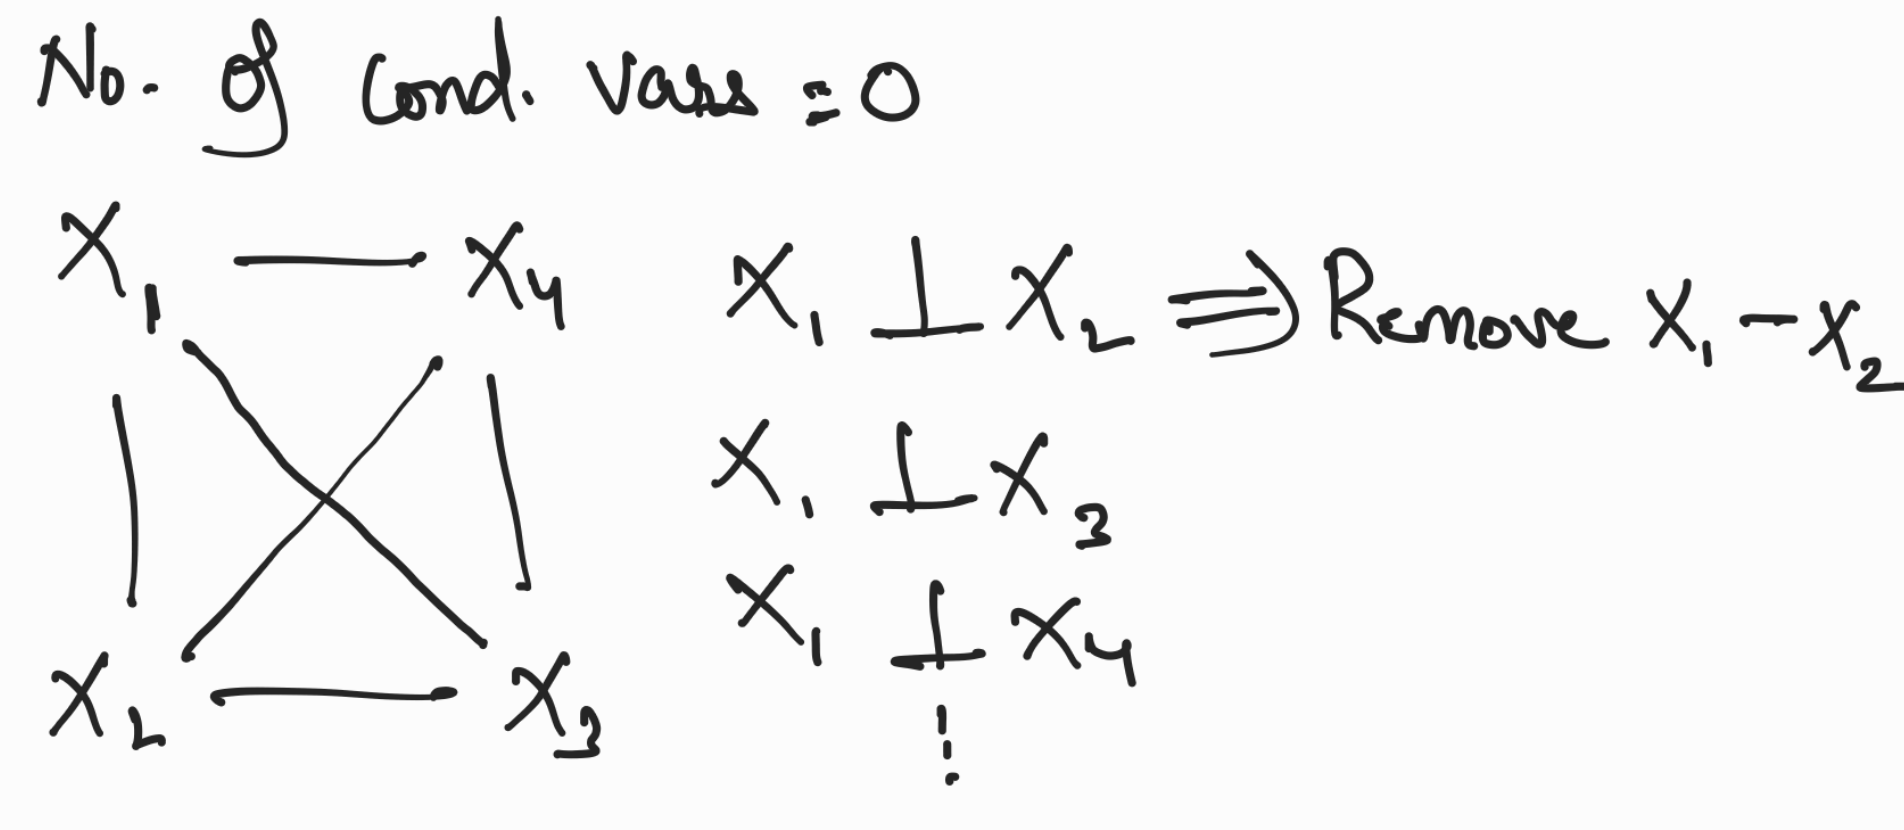
\includegraphics[scale=0.12]{imgs/example2.png}
	\end{figure}
\end{frame}

\begin{frame}
	\begin{figure}
		\centering
		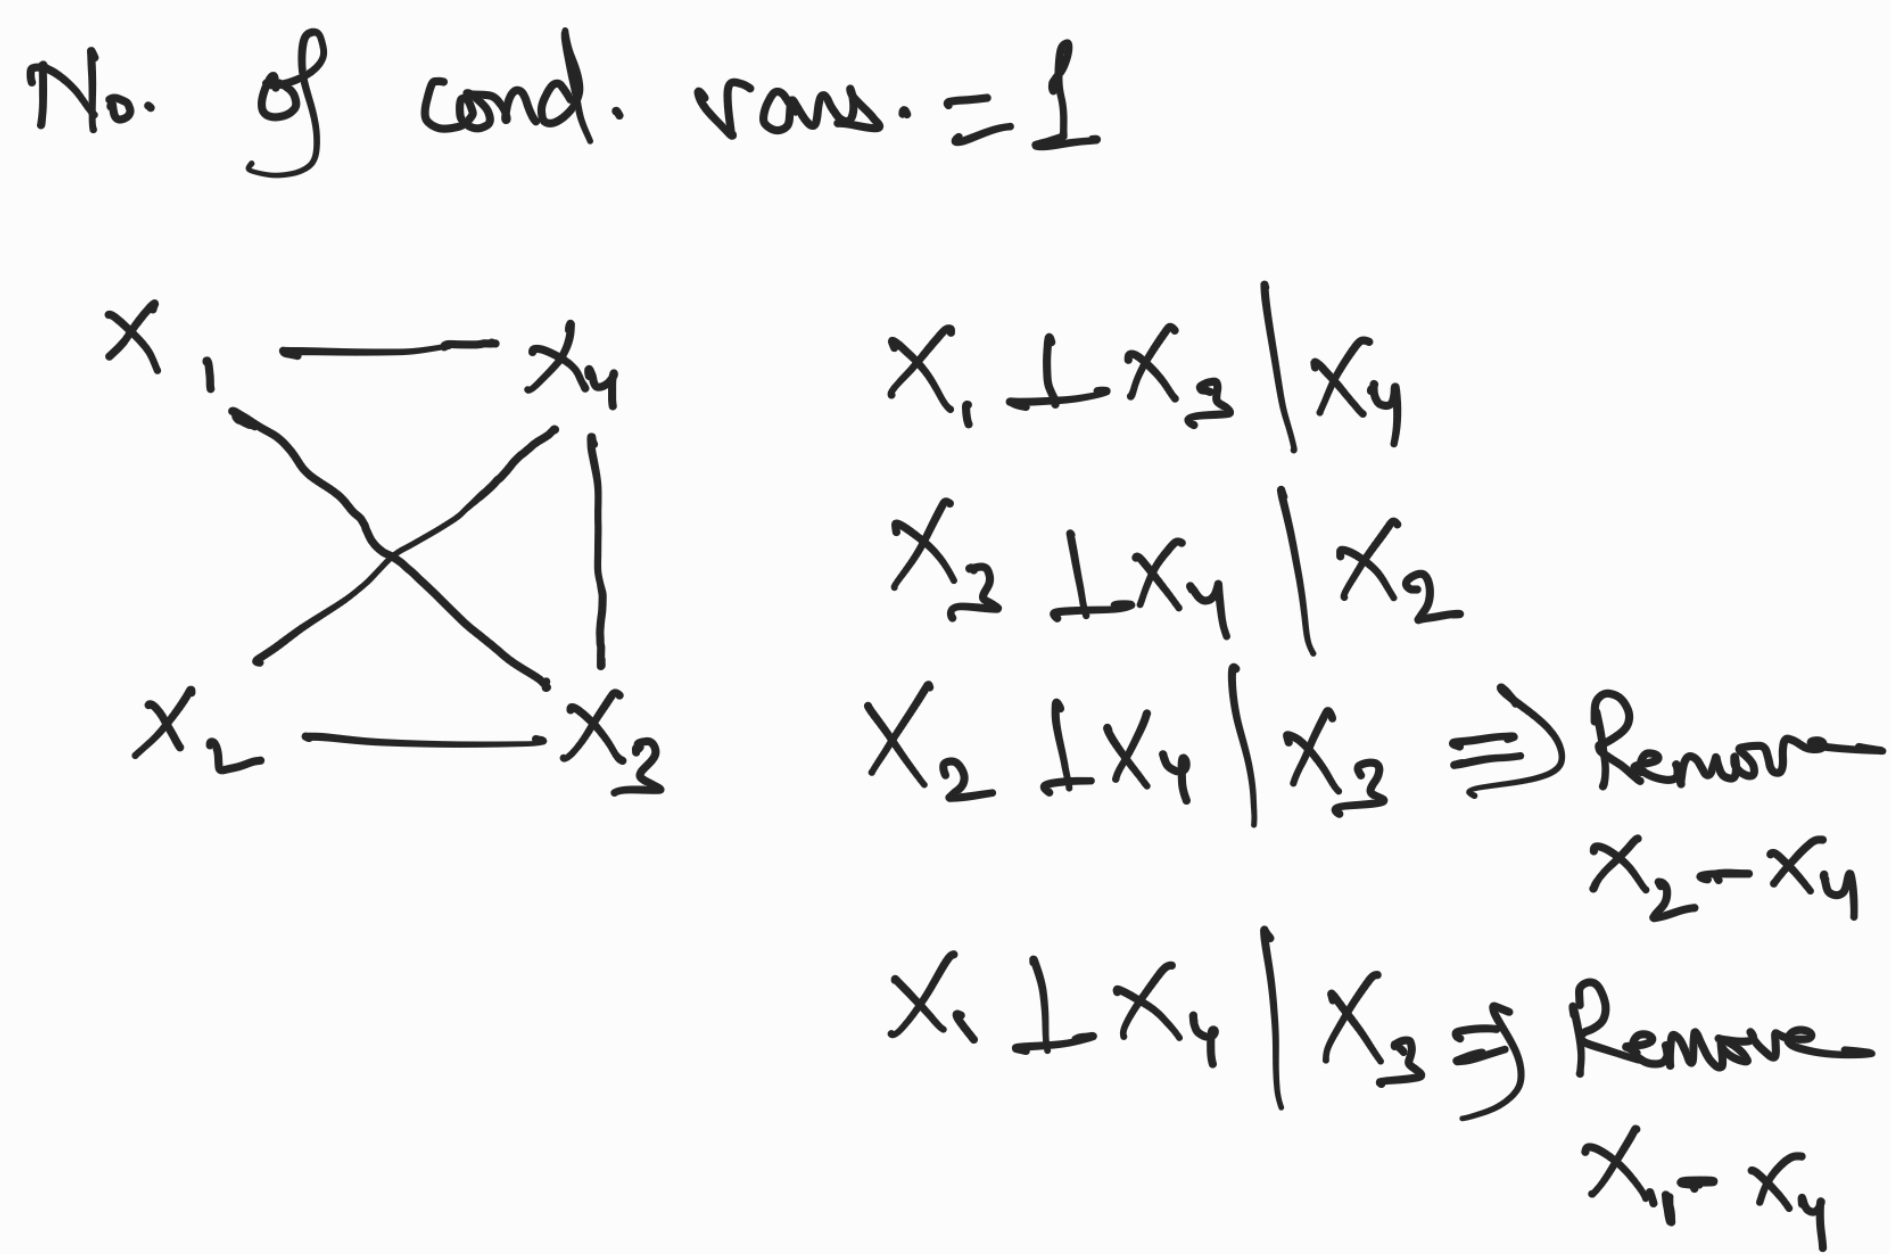
\includegraphics[scale=0.1]{imgs/example3.png}
	\end{figure}
	\begin{figure}
		\centering
		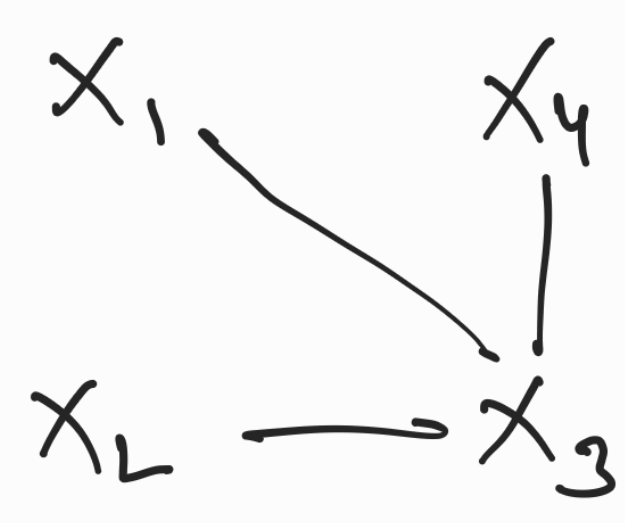
\includegraphics[scale=0.1]{imgs/example4.png}
	\end{figure}

	\center Edges are then oriented using Meek's rule.
\end{frame}

\begin{frame}{CI Testing in Data}
	Statistical tests are used to test CIs in data. Typically,
	\begin{equation*}
		\begin{split}
			H_0 &: X \ci Y \rvert Z \\
			H_A &: X \not \ci Y \rvert Z
		\end{split}
	\end{equation*}
	\vspace{2em}
	\center (p-value $ > \alpha $ ) $ \implies X \ci Y \rvert Z  \implies $ Remove Edge
\end{frame}

\begin{frame}{Problems With This Testing}
	\begin{itemize}
		\item Estimated Structures are usually too sparse, i.e., missing too many edges compared to the ground truth.
		\item Much statistical theory has been dedicated to controlling false positives. in the sense of false edge inclusion such as multiple testing adjustments, limits on false discovery rate.
		\item In practice, easy to achieve very few false edge inclusion.
		\item However, it is difficult to achieve low rates of error for false edge exclusions (high recall).
		\item Bias is causal effect estimates is largely driven by high rates of wrongly excluded edges.
	\end{itemize}
\end{frame}

\begin{frame}{Two Settings For Structure Learning Applications}
	\begin{itemize}
		\item Moderate-dimensional setting, more than $ 4 $ variables but less than hundreds.
		\item Causal graph could be partially known.
		\item Sparsity should not be assumed.
	\end{itemize}
\end{frame}

\begin{frame}{Denser Models for Epidemiological Setting}
\end{frame}

\begin{frame}{Effect Estimation in Denser Graph}
	\begin{figure}
		\centering
		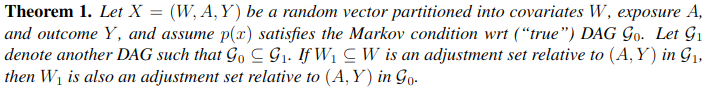
\includegraphics[scale=0.4]{imgs/theorem1.png}
	\end{figure}
	\begin{itemize}
		\item Using a super-DAG of the true DAG to select an adjustment set will always be valid.
	\end{itemize}
\end{frame}

\begin{frame}{Reformulating CI Test Hypothesis}
	\begin{itemize}
		\item $ \theta_{ij.S} $: Some measure of association between $ X_i $ and $ X_j $ given $ X_S $.
		\item $ \delta $: User chosen threshold.
	\end{itemize}

	\begin{equation*}
		\begin{split}
			H_0&: \rvert \theta_{ij.S} \rvert \ge \delta \\
			H_A&: \rvert \theta_{ij.S} \rvert < \delta \\
		\end{split}
	\end{equation*}

	\begin{itemize}
		\item $ H_0 $ implies dependence.
		\item Remove edge when $ H_0 $ is rejected.
	\end{itemize}
\end{frame}

\begin{frame}{Test Using Partial Correlation}
	\center When variables are multivariate Gaussian, Pearson's partial correlation.
	\vspace{1em}
	\begin{equation*}
		\begin{split}
			H_0&: \rvert \rho_{ij.S} \rvert \ge \delta \\
			H_A&: \rvert \rho_{ij.S} \rvert < \delta \\
		\end{split}
	\end{equation*}

	\begin{equation*}
		\begin{split}
			\textnormal{Fisher's z-transform: }& z(\hat{\rho}_{ij.S}) = \frac{1}{2} ln \frac{1+\hat{\rho}_{ij.S}}{1 - \hat{\rho}_{ij.S}} \\
			\textnormal{Property: }& \sqrt{n - \rvert S \rvert - 3}(z(\hat{\rho}_{ij.S}) - z(\rho_{ij.S})) \sim N(0, 1) \\
			\textnormal{Rejection Rule: }& \sqrt{n - \rvert S \rvert - 3}(z(\hat{\rho}_{ij.S}) - z(\delta)) \le \Phi^{-1}(\alpha) \\
			\textnormal{and } & \sqrt{n - \rvert S \rvert - 3}(z(\hat{\rho}_{ij.S}) - z(\delta)) \ge \Phi^{-1}(\alpha)
		\end{split}
	\end{equation*}
\end{frame}

\begin{frame}{Test Using Expected Conditional Covariance}
	\center{When Gaussianity assumption is not satisfied.}
	\begin{equation*}
		\begin{split}
			\Psi^*_{ij.S} &= \mathbb{E}[cov(X_i, X_j | X_S)] \\
			\sqrt{n}(\hat{\Psi}^*_{ij.S} - \Psi^*_{ij.S}) & \sim N(0, \sigma^2_{ij.S}) \\
		\end{split}
	\end{equation*}
	\begin{figure}
		\centering
		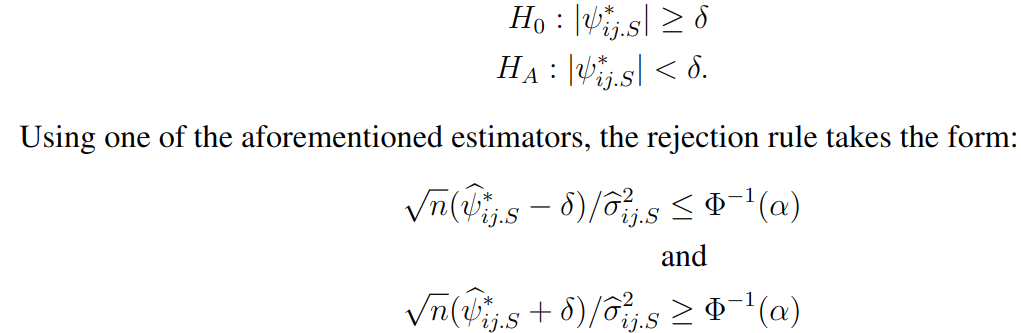
\includegraphics[scale=0.3]{imgs/test2.png}
	\end{figure}
\end{frame}

\begin{frame}{Test Using Odds Ratios}
	In case of mixed variables (continuous and binary), conditional odds ratio.

	\begin{equation*}
		\begin{split}
			\gamma_{ij.S} &= log OR(X_i, X_j \rvert X_S) \\
			\sqrt{n}(\hat{\gamma}_{ij.S} - \gamma_{ij.S}) &\sim N(0, \omega^2_{ij.S}) \\
		\end{split}
	\end{equation*}
	\begin{figure}
		\centering
		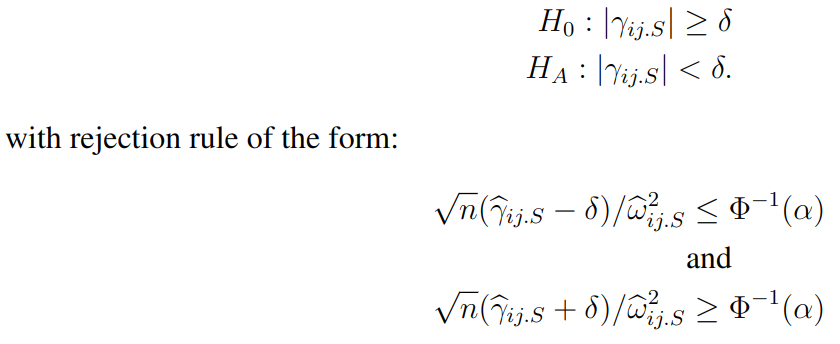
\includegraphics[scale=0.3]{imgs/test3.png}
	\end{figure}
\end{frame}

\begin{frame}{Empirical Results}
	\begin{itemize}
		\item Random graphs on $ 10 $ nodes with an expected degree of $ 7 $.
		\item Very dense graphs, $ < 10 $ missing edges.
		\item Linear data simulation with random ($ [0.5, 1.0] $) parameter value.
		\item Fixed $ \alpha = 0.05 $ for e-PC.
	\end{itemize}
\end{frame}

\begin{frame}{Empirical Results: Recall}
	\begin{figure}
		\centering
		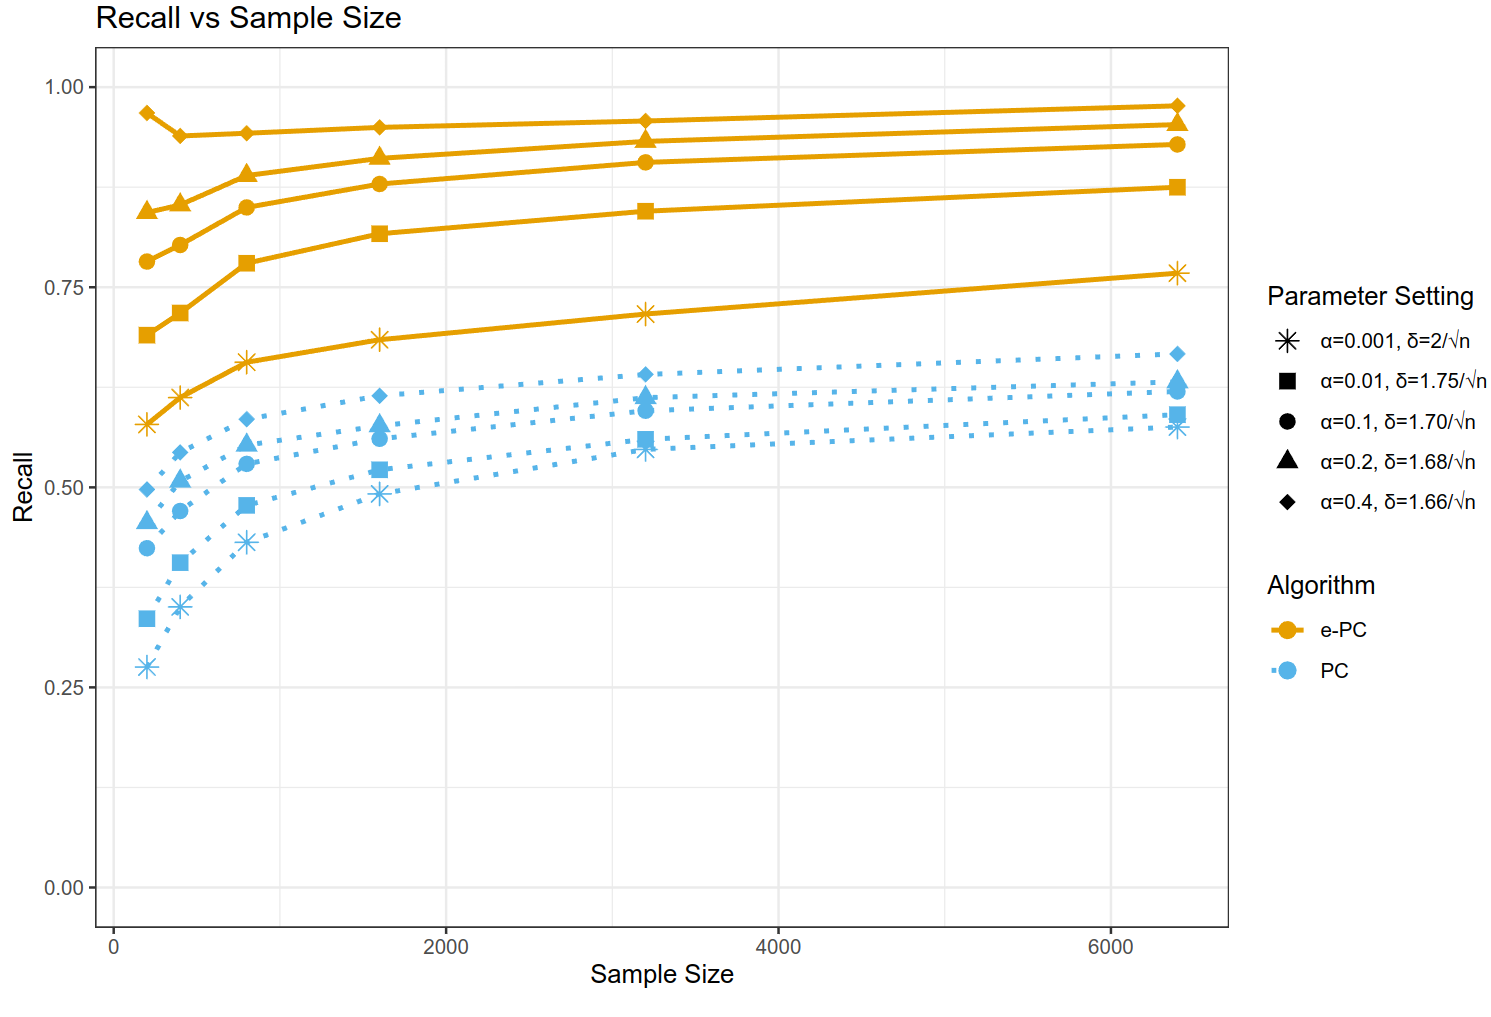
\includegraphics[scale=0.2]{imgs/recall.png}
	\end{figure}
\end{frame}

\begin{frame}{Empirical Results: Precision}
	\begin{figure}
		\centering
		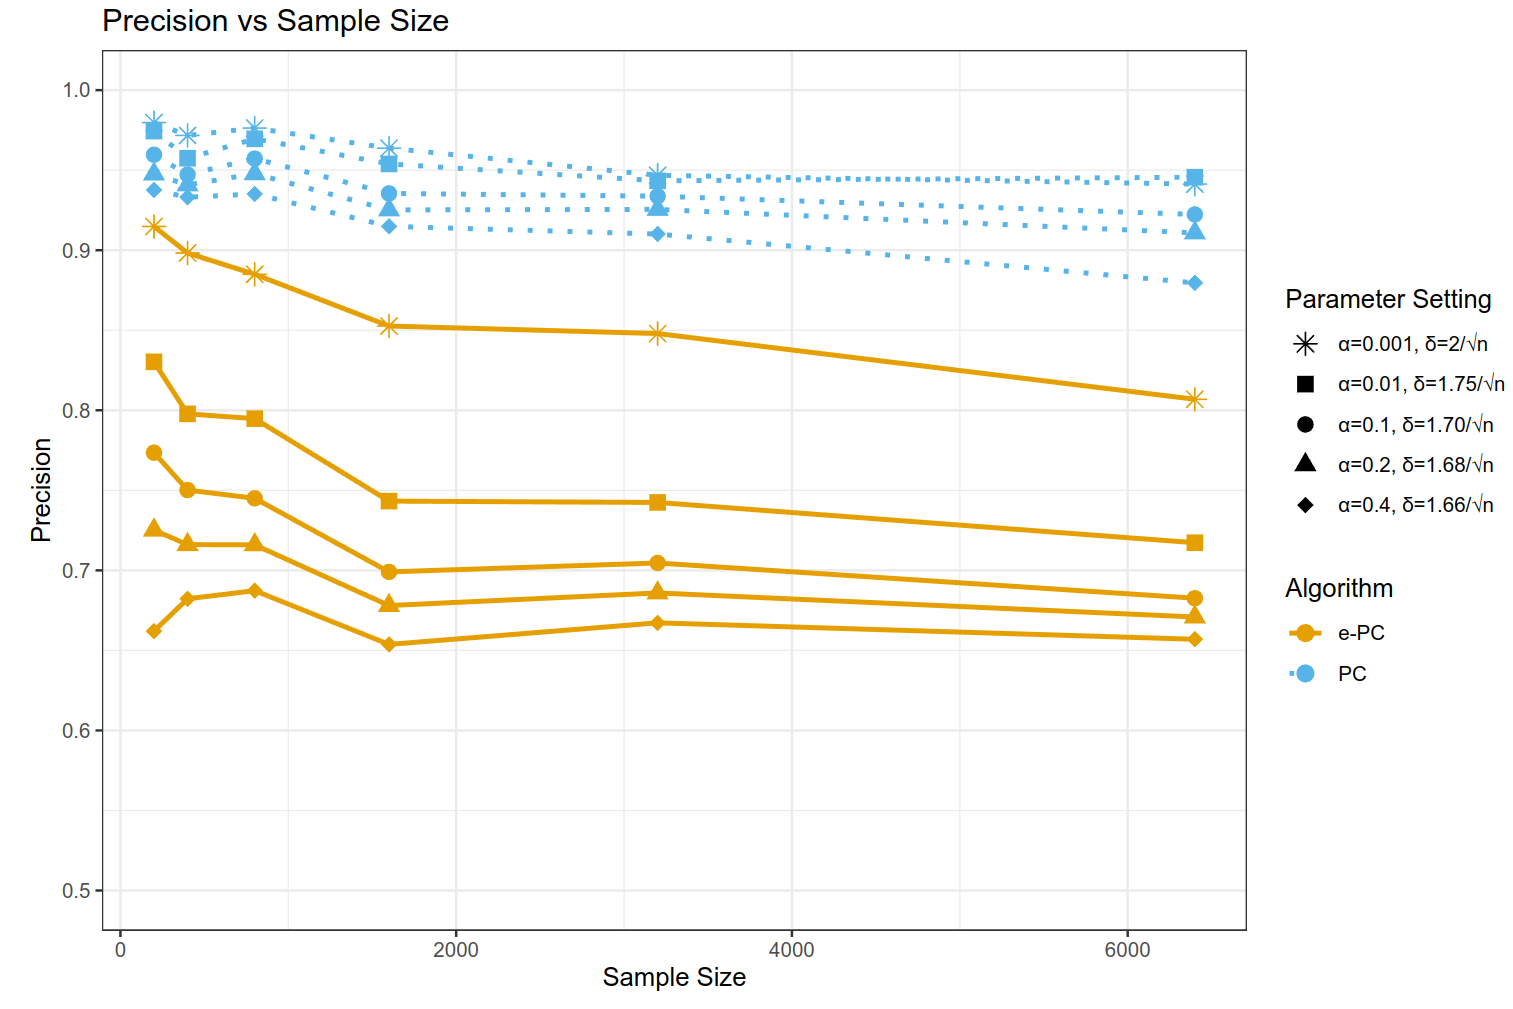
\includegraphics[scale=0.2]{imgs/precision.png}
	\end{figure}
\end{frame}

\begin{frame}{Empirical Analysis: Comparison}
	\begin{figure}
		\centering
		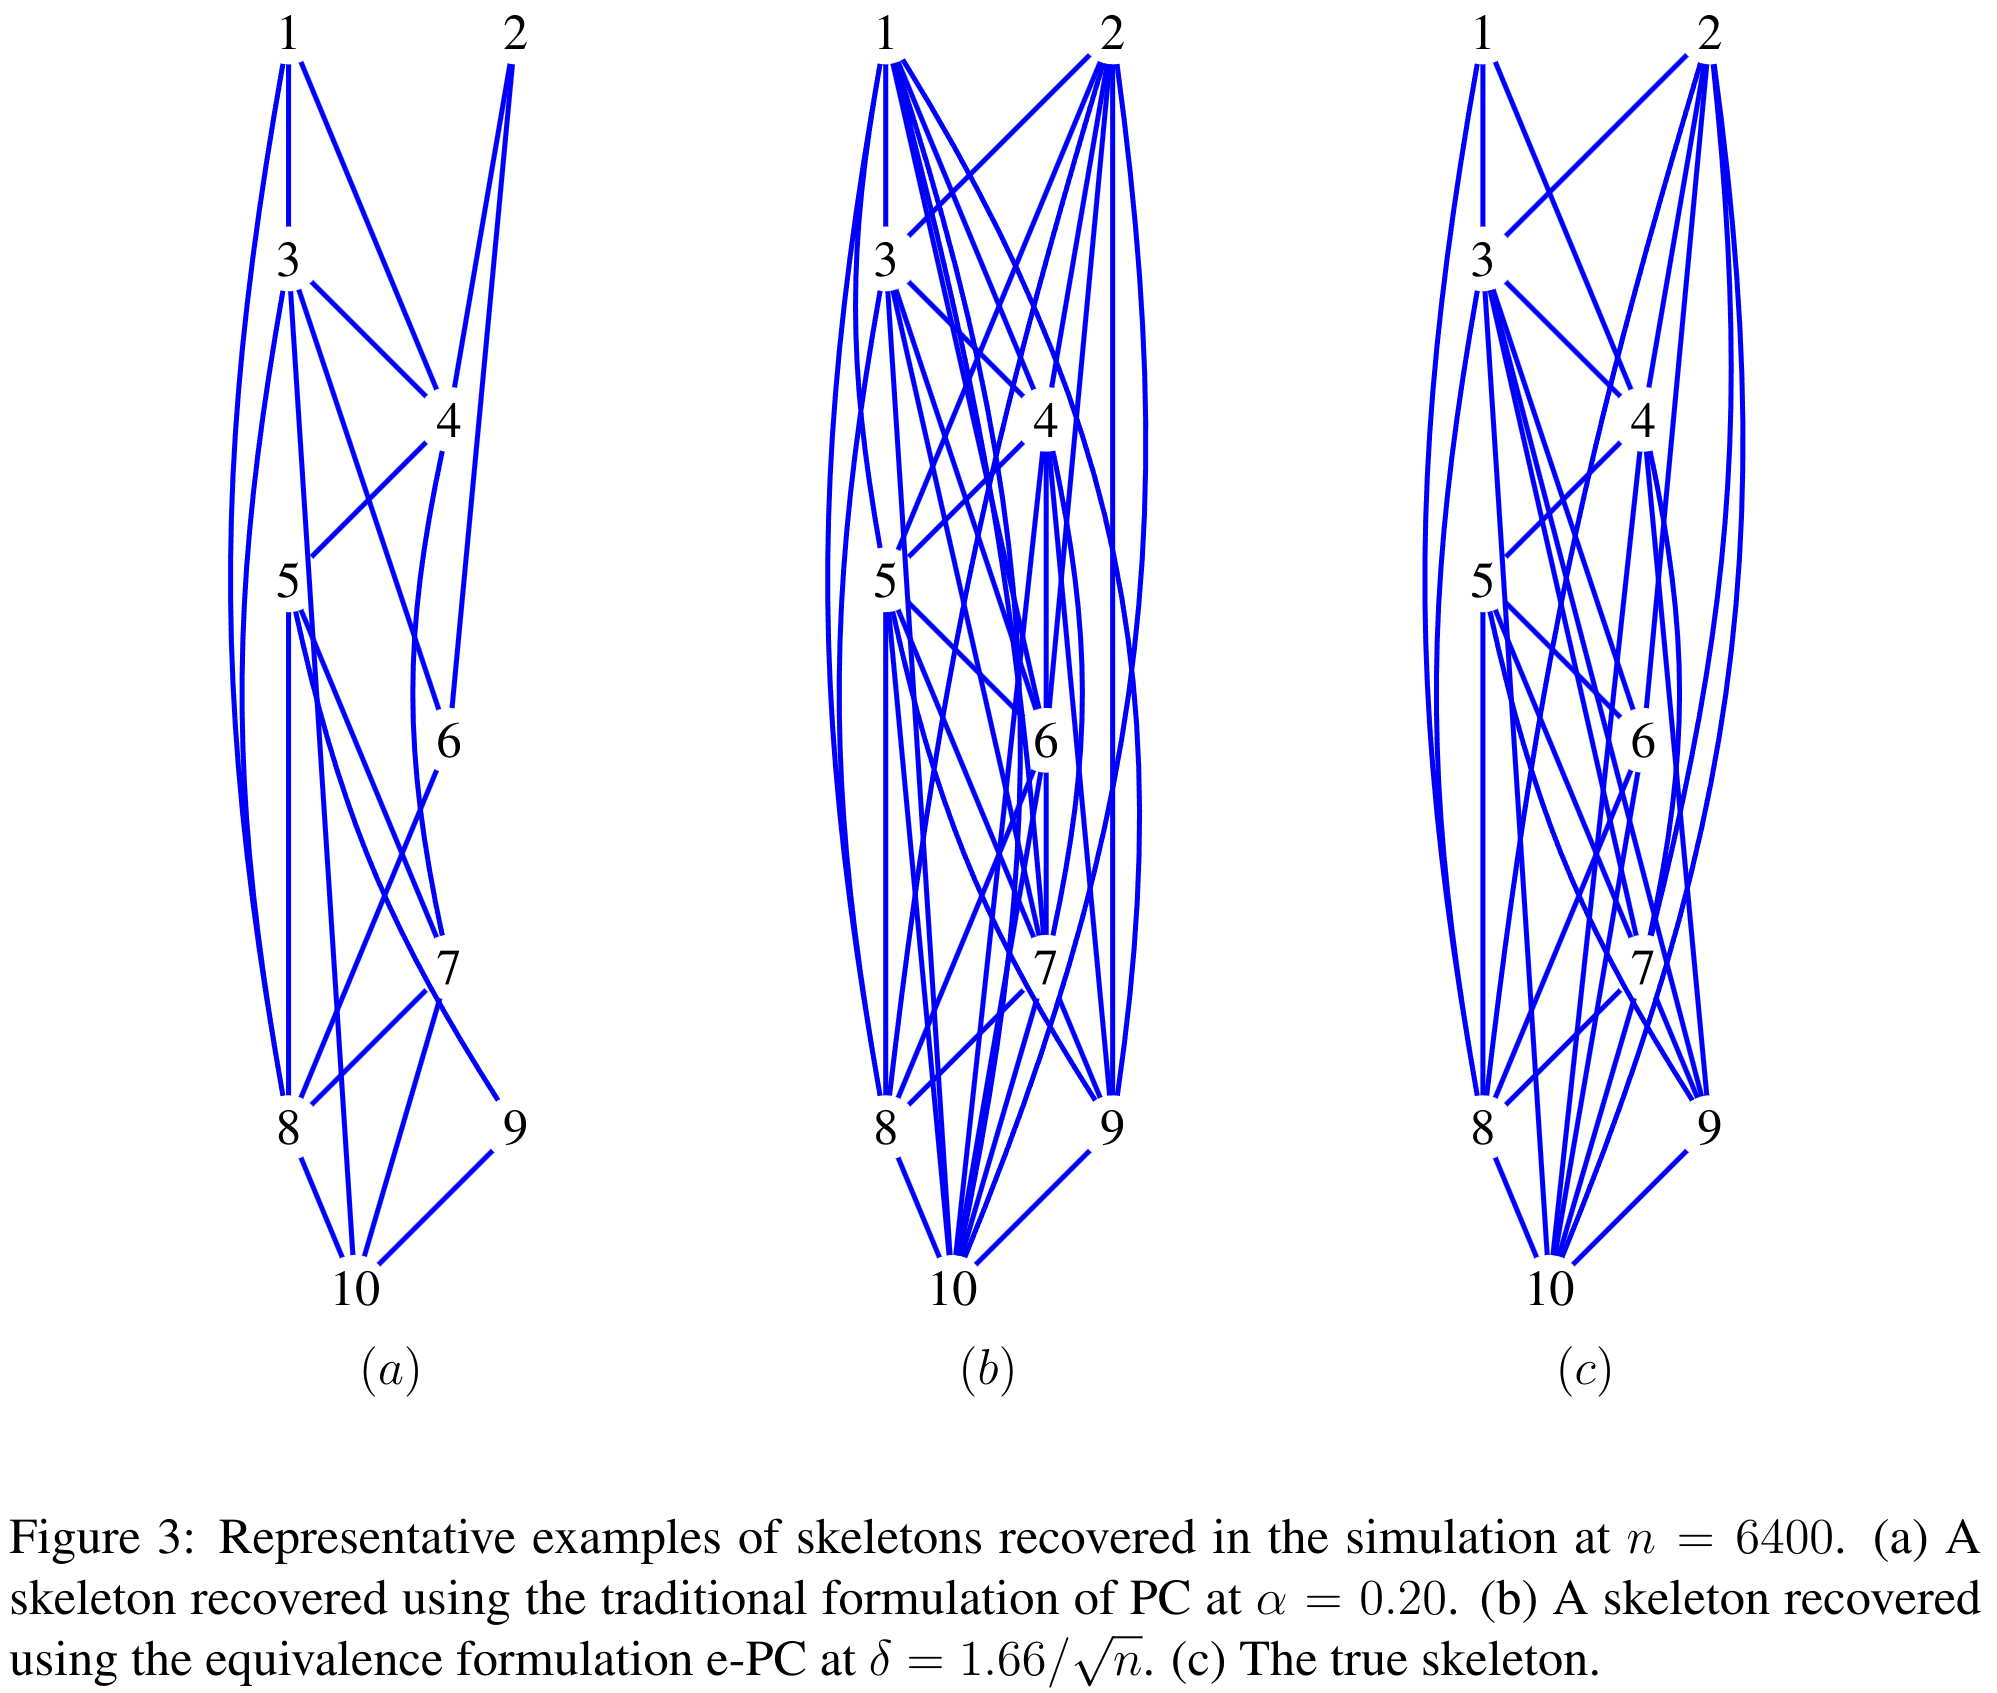
\includegraphics[scale=0.12]{imgs/empirical_compare.png}
	\end{figure}
\end{frame}

\begin{frame}{Conclusion}
	\begin{itemize}
		\item Previous approaches have been 
	\end{itemize}
\end{frame}

\end{document}
